% EE6483 Mini Project (Option 1) report. Master file, integrated by member A.
% Each section lives in sections/<id>.tex; the owner of each file is noted at
% its top. Compile: latexmk -xelatex main.tex  (or upload the report/ folder to Overleaf)
\documentclass[11pt,a4paper]{article}
\usepackage[margin=2.2cm]{geometry}
\usepackage{fontspec}
\setmainfont{Times New Roman}
\usepackage{amsmath,amssymb}
\usepackage{graphicx}
\usepackage{float}
\usepackage{booktabs}
\usepackage{tabularx}
\usepackage{multirow}
\usepackage{array}
\usepackage{xcolor}
\usepackage{caption}
\usepackage{subcaption}
\usepackage{enumitem}
\usepackage{tikz}
\usetikzlibrary{positioning,arrows.meta,shapes.geometric,fit}
\usepackage[numbers,sort&compress]{natbib}
\usepackage[colorlinks=true,linkcolor=blue!50!black,citecolor=blue!50!black,urlcolor=blue!50!black]{hyperref}

\graphicspath{{figures/}}
\setlist{itemsep=2pt,topsep=3pt}
\newcolumntype{Y}{>{\raggedright\arraybackslash}X}
% \tbd{...}: placeholder for numbers/text another member still has to supply.
\newcommand{\tbd}[1]{\textcolor{red}{[TBD: #1]}}

\title{EE6483 Artificial Intelligence and Data Mining\\Mini Project (Option 1): Sentiments of Product Reviews}
\author{Team 110}
\date{November 2026}

\setlength{\parindent}{0pt}
\setlength{\parskip}{4pt}
\begin{document}
\maketitle

\section*{Group members and contributions}
\begin{table}[h]
\centering
\begin{tabularx}{\textwidth}{l l Y}
\toprule
Member & Matric no. & Contribution \\
\midrule
MENG XIANGYU & G2607496E & Shared code (\texttt{common.py}, data split, evaluation), TF-IDF baselines, noisy-label experiment, resource/accuracy analysis; report (a)(1), (b), (g), (i); report integration. \\
WU DAYU & G2603624F & GloVe features, averaged-GloVe + LR, BiLSTM model and tuning; report (a)(2), (a)(4), (d), (h). \\
YIN JIYANG & G2605135H & RoBERTa fine-tuning, ensemble and final submission, error analysis; report (a)(3), (c), (e), (f); README. \\
\bottomrule
\end{tabularx}
\end{table}
All members contributed papers to the literature table in (a)(2) and cross-reviewed each other's sections.

\tableofcontents
\newpage

\section{(a) Literature survey}
% Owner: member A.
\subsection{(a)(1) Problem definition, challenges and solution types}

\paragraph{Problem definition.}
Sentiment analysis, also called opinion mining, is the computational study of the opinions, sentiments and emotions that people express in text~\cite{pang2008opinion,liu2012sentiment}.
Liu~\cite{liu2012sentiment} formalises an opinion as a quintuple $(e, a, s, h, t)$: an entity $e$, one of its aspects $a$, the sentiment $s$ towards that aspect, the opinion holder $h$ and the time $t$.
This project is the simplest instance of that definition: \emph{document-level binary polarity classification}.
The entity is the purchased product and the holder is the reviewer, both implicit, and each review receives one label for the whole document.
Given a review $x$, we learn a classifier $f(x) \approx P(y{=}1 \mid x)$, where $y=1$ is positive and $y=0$ is negative, and predict $\hat y = \mathbb{1}[f(x) \ge \tau]$ for a decision threshold $\tau$.
Neutral or irrelevant reviews are not modelled.

\paragraph{Granularity.}
Sentiment can be analysed at three levels of granularity:
\begin{itemize}
  \item \emph{Document level}: one label per review, as in this project~\cite{pang2002thumbs}.
  \item \emph{Sentence level}: usually a subjectivity filter followed by polarity classification.
  \item \emph{Aspect level}: aspect-based sentiment analysis (ABSA) extracts aspects such as ``fit'' or ``fabric'' and assigns a polarity to each~\cite{hu2004mining,pontiki2014semeval}.
\end{itemize}
Related tasks use finer label sets, such as the five-point scale of the Stanford Sentiment Treebank~\cite{socher2013recursive}, or emotion categories.

\paragraph{Challenges.}
The main difficulties, each illustrated with what we observe in our data:
\begin{enumerate}
  \item \textbf{Negation and contrast.} Words such as ``not'', ``never'' and ``but'' change the polarity of the words around them. In ``Not bad for just a shirt'' (from our test set), ``bad'' signals a negative review, yet the review is mildly positive. A bag-of-words model loses the word order needed to resolve this.
  \item \textbf{Implicit sentiment, sarcasm and irony.} Many reviews contain no explicit opinion word (``the seam came apart after one wash''), or say the opposite of what they mean.
  \item \textbf{Mixed polarity.} A review may praise one aspect and criticise another. The document label then depends on which aspect the reviewer weighs more.
  \item \textbf{Domain dependence.} The polarity of a word depends on the domain. ``Small'' is negative for a hotel room and often positive for a phone, and ``unpredictable'' is positive for a film plot but negative for a car's steering. Classifiers trained on one product category therefore degrade on another~\cite{turney2002thumbs,blitzer2007biographies}.
  \item \textbf{Class imbalance.} Product reviews are mostly positive: 85.4\% of our training reviews are positive and 14.6\% negative. Predicting ``positive'' for every review already gives 85.4\% accuracy, so we report Macro-F1 and the F1 of the negative class alongside accuracy.
  \item \textbf{Noisy and informal text.} Reviews contain typos, slang, emoticons and very different lengths. Our training reviews have a median of 42 words, but the longest has 1{,}066. When star ratings are used as labels, some labels disagree with the text, which is the problem studied in (i).
\end{enumerate}

\paragraph{Solution types under different settings.}
Table~\ref{tab:a1-settings} organises common approaches along the three axes named in the assignment.

\emph{Supervised versus unsupervised.}
Supervised methods learn from labelled reviews. They range from Naive Bayes, maximum-entropy and SVM classifiers on bag-of-words features~\cite{pang2002thumbs}, and their strong NB-SVM variant~\cite{wang2012baselines}, through convolutional and recurrent networks over word embeddings~\cite{kim2014convolutional,socher2013recursive,zhang2018deep}, to fine-tuning pre-trained Transformers such as BERT and RoBERTa~\cite{devlin2019bert,liu2019roberta}.
Unsupervised, lexicon-based methods need no labels:
\begin{itemize}
  \item scoring phrases by their association with seed words such as ``excellent'' and ``poor''~\cite{turney2002thumbs};
  \item looking words up in a sentiment lexicon such as SentiWordNet~\cite{baccianella2010sentiwordnet};
  \item rule-based scoring with VADER~\cite{hutto2014vader}.
\end{itemize}
They transfer easily across domains but are usually less accurate than supervised models.
Between the two extremes lie weakly supervised methods. Distant supervision uses emoticons or star ratings as noisy labels~\cite{go2009twitter}, and semi-supervised methods use self-training on unlabelled reviews. Zero-shot and few-shot prompting of large language models is competitive on simple binary polarity, but still falls behind fine-tuned models on fine-grained and structured sentiment tasks~\cite{zhang2023sentiment}.

\emph{Closed-set versus open-set.}
In the closed-set setting every test review belongs to one of the training classes, here positive or negative.
In the open-set setting, test inputs may come from classes never seen in training: neutral reviews, spam, text that is not a review, or another language.
A closed-set classifier still forces each of these into ``positive'' or ``negative''.
Open-set methods add a rejection option. DOC replaces the softmax with one-vs-rest sigmoids and rejects an input when no class is confident enough~\cite{shu2017doc}. Confidence-based detection flags inputs whose maximum softmax probability is low~\cite{hendrycks2017baseline}.

\emph{Without versus with domain shift.}
When training and test data come from the same distribution, standard supervised learning applies.
Under domain shift, labelled data from a source domain (e.g.\ books) must serve an unlabelled target domain (e.g.\ kitchen appliances). Approaches include:
\begin{itemize}
  \item structural correspondence learning, which aligns domain-specific words through shared ``pivot'' features~\cite{blitzer2007biographies};
  \item stacked denoising autoencoders that learn domain-invariant representations~\cite{glorot2011domain};
  \item domain-adversarial training (DANN)~\cite{ganin2016domain};
  \item continued pre-training of the language model on target-domain text~\cite{gururangan2020dont}.
\end{itemize}
These methods are the basis of our answer to (h).

\begin{table}[t]
\centering
\caption{Solution types for sentiment classification under different settings. Our project is marked with $\star$.}
\label{tab:a1-settings}
\small
\begin{tabularx}{\textwidth}{l Y Y}
\toprule
Setting & Typical methods & Strengths / limitations \\
\midrule
Supervised $\star$ & BoW + NB/LR/SVM~\cite{pang2002thumbs,wang2012baselines}; CNN/RNN over embeddings~\cite{kim2014convolutional,socher2013recursive}; fine-tuned Transformers~\cite{devlin2019bert,liu2019roberta} & Most accurate when labelled in-domain data exist; needs labels and is domain-specific. \\
Unsupervised & Seed-word association~\cite{turney2002thumbs}; lexicons~\cite{baccianella2010sentiwordnet}; rules (VADER)~\cite{hutto2014vader} & No labels needed and interpretable; misses context, domain-specific terms and sarcasm. \\
Weak / semi-supervised & Distant labels from emoticons or ratings~\cite{go2009twitter}; self-training; LLM prompting~\cite{zhang2023sentiment} & Cheap labels at scale; labels are noisy (see (i)). \\
\midrule
Closed-set $\star$ & Softmax over a fixed label set & Simple; inputs from unseen classes are forced into a known class. \\
Open-set & One-vs-rest rejection (DOC)~\cite{shu2017doc}; confidence thresholds~\cite{hendrycks2017baseline} & Can reject neutral or irrelevant inputs; needs extra thresholds. \\
\midrule
No domain shift $\star$ & Standard train/validation/test protocol & Validation accuracy predicts test accuracy. \\
Domain shift & SCL pivots~\cite{blitzer2007biographies}; denoising autoencoders~\cite{glorot2011domain}; DANN~\cite{ganin2016domain}; domain-adaptive pre-training~\cite{gururangan2020dont} & Uses unlabelled target text; gains depend on how far apart the domains are. \\
\bottomrule
\end{tabularx}
\end{table}

\paragraph{Our setting.}
The project is \emph{supervised, closed-set and in-domain}.
Training and test reviews come from the same product-review distribution; 101 of the 1{,}851 test reviews even appear verbatim in the training set.
The data are imbalanced, and the labels may contain some noise.
We therefore build supervised classifiers. A TF-IDF linear model serves as the baseline, and sequence models and pre-trained language models serve as improvements; (a)(4) motivates this choice.
We use threshold tuning and Macro-F1 to handle the imbalance.

% Owner: member B. Append A/C entries after checking for duplicates.
\subsection{(a)(2) Recent papers}
Table~\ref{tab:recent-sentiment} covers domain adaptation, sentiment-aware
representation learning, and evaluation under distribution shift. The
published results use different benchmarks and protocols.

\begin{table}[htbp]
\centering
\caption{Selected recent work on sentiment classification and transfer.}
\label{tab:recent-sentiment}
\small
\renewcommand{\arraystretch}{1.08}
\begin{tabularx}{\textwidth}{@{}l >{\raggedright\arraybackslash}p{.16\textwidth}
  >{\raggedright\arraybackslash}p{.20\textwidth} Y Y@{}}
\toprule
Year & Method & Data & Contribution & Reported result \\
\midrule
2021 & UDALM~\cite{karouzos2021udalm} & Amazon Reviews, 12 transfers &
Joint source classification and target masked language modelling &
91.74\% accuracy, 1.11 percentage points above the prior comparison. \\
2022 & Memory-based contrastive learning~\cite{tan2022memory} &
Two Amazon review datasets and a rumour dataset &
Queue-based supervised contrastive learning for unseen domains &
Improved over the tested domain adaptation methods. \\
2022 & Mere contrastive learning~\cite{luo2022mere} &
Amazon Reviews and FDU-MTL &
In-batch negatives separate classes in representation space &
90.39\% mean accuracy over 12 Amazon transfers. \\
2022 & Multi-domain TSA~\cite{toledoronen2022multi} &
Yelp for self-training, three target evaluation datasets &
Augments training with weakly labelled examples across domains &
Showed gains across target datasets. \\
2024 & SentiEval~\cite{zhang2023sentiment} &
26 datasets over 13 sentiment tasks &
Compares prompted LLMs and task-trained smaller models &
Simple classification was more favourable to LLMs than fine-grained structured tasks. \\
2024 & SoftMCL~\cite{wang2024softmcl} &
Sentence- and aspect-level sentiment and other affective tasks &
Uses soft valence and a momentum queue during pretraining &
Showed benefits across several sentiment tasks. \\
2025 & Synthetic instructions~\cite{zhao2025instruction} &
12 sentiment benchmarks including Amazon, Yelp and IMDb &
Builds instruction examples without labelled review instances &
Reported a 5.1-point gain over more complex instruction tuning methods. \\
2025 & BESSTIE~\cite{srirag2025besstie} &
Google Place and Reddit texts in three English varieties &
Tests sentiment and sarcasm across varieties &
Performance fell on Indian English, especially for sarcasm. \\
\bottomrule
\end{tabularx}
\end{table}

Domain adaptation studies suggest using hotel text during training even
without ratings. Cross-variety evaluation and the LLM comparisons also
motivate keeping a held-out target sample when testing transfer. For the
present product-review task, we compare sparse lexical and dense embedding
models on the same split before drawing conclusions about transfer.

% Owner: member C. Placeholder created by A; replace with the section text.
\subsection{(a)(3) Top research groups}
\tbd{member C}

% Owner: member B. Placeholder created by A; replace with the section text.
\subsection{(a)(4) Baseline choice and motivation}
\tbd{member B}


\section{(b) Feature format and data preprocessing}
\subsection{Feature formats and pipeline}
We compare three feature formats of increasing cost, one per model line, so that Section~\ref{sec:formats} can measure the trade-off directly:
\begin{enumerate}
  \item \textbf{Sparse bag-of-n-grams with TF-IDF weighting}, used by linear classifiers;
  \item \textbf{static pre-trained word embeddings} (300-dimensional GloVe\cite{pennington2014glove}), used by an averaged-embedding classifier and by a BiLSTM;
  \item \textbf{subword tokens fed to a pre-trained Transformer} (RoBERTa-base), whose contextual representation is fine-tuned end-to-end. This is the format of our final model.
\end{enumerate}
Figure~\ref{fig:b-pipeline} summarizes the pipeline. All three formats share the loading, auditing, splitting and cleaning steps described below.

\begin{figure}[tbp]
\centering
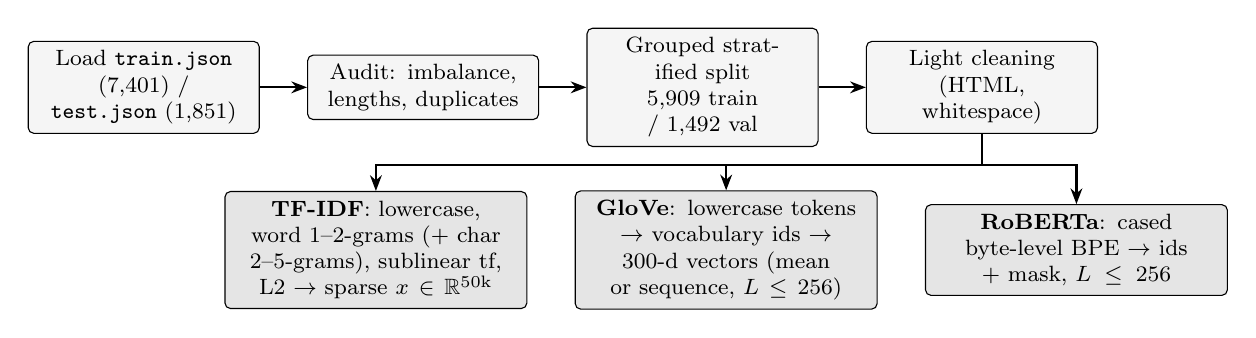
\begin{tikzpicture}[
  node distance=4mm and 6mm,
  box/.style={draw, rounded corners=2pt, align=center, font=\footnotesize, minimum height=8mm, text width=27mm, fill=gray!8},
  fbox/.style={box, text width=36mm, fill=gray!20},
  arr/.style={-{Stealth[length=2mm]}, thick}]
\node[box] (load) {Load \texttt{train.json}\\(7{,}401) / \texttt{test.json} (1{,}851)};
\node[box, right=of load] (audit) {Audit: imbalance,\\lengths, duplicates};
\node[box, right=of audit] (split) {Grouped stratified split\\5{,}909 train / 1{,}492 val};
\node[box, right=of split] (clean) {Light cleaning\\(HTML, whitespace)};
\node[fbox, below=9mm of audit, xshift=-6mm] (tfidf) {\textbf{TF-IDF}: lowercase, word 1--2-grams (+ char 2--5-grams), sublinear tf, L2 $\rightarrow$ sparse $x\in\mathbb{R}^{50\text{k}}$};
\node[fbox, right=of tfidf] (glove) {\textbf{GloVe}: lowercase tokens $\rightarrow$ vocabulary ids $\rightarrow$ 300-d vectors (mean or sequence, $L\le256$)};
\node[fbox, right=of glove] (bpe) {\textbf{RoBERTa}: cased byte-level BPE $\rightarrow$ ids + mask, $L\le256$};
\draw[arr] (load) -- (audit);
\draw[arr] (audit) -- (split);
\draw[arr] (split) -- (clean);
\draw[arr] (clean.south) |- ++(0,-4mm) -| (tfidf.north);
\draw[arr] (clean.south) |- ++(0,-4mm) -| (glove.north);
\draw[arr] (clean.south) -- ++(0,-4mm) -| (bpe.north);
\end{tikzpicture}
\caption{Data preprocessing pipeline. Every vectorizer, vocabulary and model is fitted on the training part only; the validation split is used only for model selection and the test set only for the final predictions.}
\label{fig:b-pipeline}
\end{figure}

\subsection{Data audit}
Both files are read as JSON tables.
The training set has 7{,}401 reviews with a binary label (6{,}319 positive, 1{,}082 negative). The test set has 1{,}851 unlabeled reviews. No review is missing or empty.
Review length varies widely: the median is 42 words, 75\% of reviews have at most 70 words, 97\% at most 178, and the longest has 1{,}066 words.
We also checked for duplicates, comparing texts after lower-casing and collapsing whitespace:
\begin{itemize}
  \item 154 distinct texts occur more than once in the training set, covering 373 rows, and every copy of a text has the same label;
  \item 101 test reviews are identical to a training review;
  \item 21 test reviews duplicate another test review.
\end{itemize}

\subsection{Grouped, stratified validation split}
Every model is tuned on one shared validation split.
If duplicates were split at random, copies of the same review would land on both sides, and the validation score would partly measure memorization.
We therefore group rows by their normalized text and take fold~0 of a 5-fold \texttt{StratifiedGroupKFold} (seed 42).
This yields 5{,}909 training and 1{,}492 validation reviews. The validation set contains 218 negatives (14.6\%, the same ratio as the full set), and no text appears on both sides.
Cross-validation inside the training part, including the internal folds used to calibrate the SVM, uses the same grouping.
The test set is used only to produce \texttt{submission.csv}.

\subsection{Text cleaning}
We unescape HTML entities, collapse runs of whitespace and strip leading and trailing spaces.
We deliberately do \emph{not}:
\begin{itemize}
  \item remove stop words, because standard stop lists contain ``not'', ``no'' and ``but'', which carry sentiment;
  \item stem, or strip punctuation such as ``!'' and ``?''.
\end{itemize}
Text is lower-cased for TF-IDF and GloVe, and kept in its original case for RoBERTa, whose tokenizer is case-sensitive.

\subsection{TF-IDF features (L1)}
The text is tokenized with a pattern that keeps single-character tokens (e.g.\ the ``t'' of ``don't'') as well as ``!'' and ``?''.
We extract unigrams and bigrams; bigrams capture short negations such as ``not good'' and ``not worth''.
Each term $t$ in review $d$ is weighted with sublinear term frequency and smoothed inverse document frequency,
\begin{equation}
  w_{t,d} = \bigl(1 + \log \mathrm{tf}_{t,d}\bigr)\cdot\Bigl(\log\frac{1+N}{1+\mathrm{df}_t} + 1\Bigr),
\end{equation}
where $N$ is the number of training reviews and $\mathrm{df}_t$ the number of reviews containing $t$. Each review vector is then L2-normalized.
The vectorizer is fitted on the training rows only.
Three settings were tuned by grouped 5-fold cross-validation:
\begin{itemize}
  \item the minimum document frequency (1, 2 or 3);
  \item the vocabulary cap (10k, 30k, 50k or unlimited);
  \item whether to append character 2--5-grams, which can absorb misspellings.
\end{itemize}
The selected representation has 50{,}000 word 1--2-gram features. It is very sparse: 86 non-zeros per review on average, a density of 0.17\%.

\subsection{Static word embeddings (L2)}
The L2 tokenizer lowercases and unescapes the text, retains contractions and
the punctuation tokens \texttt{!} and \texttt{?}, and keeps up to 256 tokens.
The vocabulary is built only on the training portion, with minimum frequency
two and special \texttt{<pad>} and \texttt{<unk>} entries. Of 6,796 ordinary
training vocabulary entries, 6,359 have a vector in the 300-dimensional
\texttt{glove.6B} table\cite{pennington2014glove}.
On validation, 3.17\% of token occurrences map to \texttt{<unk>}, and
4.95\% have no usable pretrained vector after applying the vocabulary.
Mean GloVe averages only the covered vectors. BiLSTM gives each in-vocabulary
entry missing a GloVe vector and the shared unknown entry a random initial
vector. Padding is excluded from both directions and the pooled statistics.

\subsection{Subword tokens for a pre-trained Transformer (L3)}
After cleaning, reviews retain their original casing. RoBERTa's
byte-level BPE tokenizer converts the text to token IDs and adds the
\texttt{<s>} and \texttt{</s>} tokens. The 256-token limit includes
these special tokens. When a review is too long, the tokenizer keeps
the beginning of the text. Each batch is padded to the length of its
longest sequence, and the attention mask distinguishes input tokens
from padding. Section~\ref{sec:models} describes how the model uses the first token's
representation for classification.

\subsection{Labels and class imbalance}
Labels are used as given (0 = negative, 1 = positive).
Each model outputs $P(y{=}1\mid x)$. We report metrics at threshold~0.5 and at thresholds tuned on the validation split: one maximizing accuracy ($\tau_{\mathrm{acc}}$, used for the submission) and one maximizing Macro-F1 ($\tau_{\mathrm{F1}}$).
The RoBERTa runs used unweighted cross-entropy. Section~\ref{sec:hparams} describes the parameter settings evaluated for the other models.


\section{(c) Model}
% Owner: member C. Placeholder created by A; replace with the section text.
\tbd{member C}


\section{(d) Parameter selection}
% Owner: member B. C supplies the final Transformer tuning values.
\paragraph{Sparse baseline.}
The sparse models use grouped five-fold cross-validation within the 5,909
training reviews. The TF-IDF grid covers minimum document frequency, a
vocabulary cap and optional character features. These control the trade-off
between coverage of rare expressions and the number of features. Logistic
regression uses $C=10$ and balanced class weights with 50,000 word unigram and
bigram features. The calibrated LinearSVC selects $C=1$ without class weights,
and ComplementNB selects $\alpha=0.1$ with 10,000 features.

\paragraph{Static embedding models.}
For mean GloVe, we compare $C\in\{0.1,1,10\}$ with and without balanced class
weights. At the common threshold of 0.5, the $C=10$ balanced setting has the
highest Macro-F1 (0.7623). Its unweighted counterpart scores 0.7598 Macro-F1
and 0.8988 accuracy, versus 0.8539 accuracy with weighting. The higher negative
F1 with weighting (0.6148 versus 0.5770) explains the selection despite the
accuracy trade-off. The BiLSTM begins with Adam, learning rate $10^{-3}$, hidden width 128
per direction, dropout 0.3, trainable embeddings, and ordinary cross-entropy.
A sequential search changes learning rate ($10^{-3}$ or $5\times10^{-4}$),
hidden width (64, 128 or 256), dropout (0.3 or 0.5), embedding freezing, then
class weighting. This limits cost and isolates each comparison near the
incumbent configuration. A factorial search would be needed to estimate
interactions between settings.
The learning rate controls step size, dropout reduces overfitting, and
freezing tests whether source supervision benefits from updating GloVe.
Class weighting changes gradients during training, while threshold tuning
changes the operating point after training. Each run uses batches of 64,
gradient clipping at 1.0, up to 10 epochs and patience of two epochs.

Candidates are ranked by validation Macro-F1 at threshold 0.5. The selected
BiLSTM configuration is repeated with seeds 42, 43 and 44. We use the
standard deviation to describe run-to-run variability. Since the same
validation fold also guides tuning and early stopping, these are model-selection
scores. The unlabeled product test set is used for prediction.
For each model, the accuracy and Macro-F1 thresholds are then fitted separately
on the validation probabilities.

The sequential sweep ran seven configurations, followed by the three final fits. The selected learning rate is $0.001$, with width 128 per direction, dropout 0.3, trainable embeddings, and ordinary cross-entropy. The single-seed Macro-F1 is $0.8383\pm0.0050$ (mean and population standard deviation). The three-seed probability average reaches 0.8524 Macro-F1 at threshold 0.5. Its validation-selected thresholds are $\tau_{\mathrm{acc}}=0.500$ and $\tau_{\mathrm{F1}}=0.500$. The individual settings and scores are recorded in \texttt{outputs/bilstm/hparam\_log.csv}.

\paragraph{Transformer.}
RoBERTa-base was fine-tuned with AdamW (learning rate $2\times10^{-5}$, weight decay 0.01), unweighted cross-entropy, batch size 4, maximum length 256 and a single epoch, in fp32 with a constant learning rate.
The small learning rate is the usual choice for fine-tuning a pre-trained encoder: larger steps overwrite the pre-trained representation, while one epoch was enough to reach about 95\% validation accuracy on 5.9k reviews.
The batch size of 4 was set by the memory of the laptop GPU.
Because of the deadline, no learning-rate or loss-weighting search was run for this model; class imbalance is handled by tuning the decision threshold on the validation split instead.
Seeds 42 and 43 reached validation Macro-F1@0.5 of 0.897 and 0.884. The seed-44 run diverged to a constant prediction (Macro-F1 0.461), a known failure mode of fine-tuning without learning-rate warm-up; a linear warm-up would be the first change to make.
\tbd{C: update if seed 44 is re-run with warm-up.}


\section{(e) Test-set results}
\paragraph{Final model.}
We averaged the positive-class probabilities from the three
RoBERTa-base runs trained with 10\% warmup and linear decay. At a
threshold of 0.5, the population standard deviation of single-run
Macro-F1 decreased from 20.27 percentage points under the original
schedule to 0.43 percentage points across the same three seeds. On the
validation set, the final RoBERTa ensemble achieved 92.73\% Macro-F1
after threshold selection. The 75\% RoBERTa and 25\% TF-IDF + SVM
blend achieved 92.57\% after its own threshold selection, so we used
the RoBERTa ensemble for submission.

\paragraph{Decision threshold.}
On the 1,492 labelled validation reviews, a threshold of 0.590 gave
the highest accuracy (96.25\%) and Macro-F1 (92.73\%) among the
thresholds evaluated for the RoBERTa ensemble. We applied the same
threshold to the test set, assigning label 1 to reviews with an
average positive-class probability of at least 0.590 and label 0
to the remaining reviews.

\paragraph{Test predictions.}
The table shows the predicted label distribution for the 1,851
unlabeled test reviews.

\begin{center}
\begin{tabular}{lrr}
\hline
Predicted label & Number of reviews & Share \\
\hline
Positive (1)    & 1,568             & 84.71\% \\
Negative (0)    &   283             & 15.29\% \\
\hline
Total           & 1,851             & 100.00\% \\
\hline
\end{tabular}
\end{center}

The file \texttt{submission.csv} contains the \texttt{reviews}
and \texttt{predictions} columns in the original test-set order.

\section{(f) Analysis of correctly and incorrectly classified samples}
\paragraph{Correct and incorrect predictions.}
RoBERTa matched the final human labels on 31 of the 40 sampled reviews
(77.5\%). The sample deliberately included reviews near the decision
threshold and reviews on which the models disagreed, so this accuracy
applies only to the selected reviews.

RoBERTa correctly classified reviews 274 and 99. In review 274, the
reviewer points out a limitation of the garment and still recommends
it for smoothing under clothes. That recommendation supports the
positive label. In review 99, the reviewer initially liked the bra's
shape and support, but the underwire eventually broke through. This
failure supports the negative label despite the initial praise.

RoBERTa classified review 549 as positive even though the reviewer
reported a broken boot strap and asked about returning the boots.
It classified review 1123 as negative. In that review, the cracking
and breaking described by the reviewer concerned the old plastic
luggage tags. The reviewer was satisfied with the new leather tag,
which was the product being evaluated.

\section{(g) Effect of the feature format on resources and accuracy}
% Owner: member A. Numbers come from outputs/*/metrics.json via
% src/resource_table.py and from src/tfidf_dim_study.py. Rows marked TBD are
% filled in once B and C push their outputs (rerun resource_table.py).

The feature format decides two things: what information reaches the classifier (word identity only, word similarity, or word meaning in context), and how much computation and memory are needed to obtain it.
We first compare the three formats in general terms (Table~\ref{tab:g-qual}), then report what we measured on this dataset (Table~\ref{tab:g-measured}), and finally isolate the effect of feature dimensionality inside the TF-IDF line (Table~\ref{tab:g-dims}).

\begin{table}[t]
\centering
\caption{Comparison of the three feature formats used in this project.}
\label{tab:g-qual}
\small
\begin{tabularx}{\textwidth}{l Y Y Y}
\toprule
 & TF-IDF n-grams (L1) & Static GloVe embeddings (L2) & Contextual subwords, RoBERTa (L3) \\
\midrule
Representation & Sparse, one dimension per n-gram (here 50k; 0.17\% non-zero) & Dense, 300 per token; mean-pooled or sequential & Dense, 768 per subword token, context-dependent \\
Word order / context & Only local, via bigrams & Mean: none. BiLSTM: learned sequentially & Full self-attention over 256 tokens \\
Similar words & Unrelated dimensions (``great'' vs ``excellent'') & Close in vector space & Close, and disambiguated by context \\
Out-of-vocabulary words & Dropped (2.1\% of validation tokens, 24\% of word types) & \texttt{<unk>} or random vector (\tbd{B: OOV rate}) & None: unknown words are split into subwords \\
Trainable parameters & $\approx$\,dimension $+\,1$ (50k) & Mean+LR: 301. BiLSTM: $\approx$0.8M + embeddings & $\approx$125M \\
Hardware / training cost & CPU, seconds & CPU, minutes (BiLSTM) & GPU, minutes to hours \\
Memory & Sparse matrix of a few MB & Embedding table $V\times300$ (the full GloVe file is $\approx$1\,GB) & $\approx$0.5\,GB of weights plus activations \\
Interpretability & High: one weight per n-gram & Low & Low (needs attribution methods) \\
Data needed & Moderate; benefits from more data & Less, thanks to pre-trained vectors & Least for a given accuracy; knowledge transferred from pre-training \\
\bottomrule
\end{tabularx}
\end{table}

\begin{table}[t]
\centering
\caption{Measured accuracy and resource use on the shared validation split (1{,}492 reviews, 218 negative). Training time excludes loading data and pre-trained weights. TF-IDF runs are deterministic, so their seed standard deviation is 0. Neural models are averaged over seeds 42/43/44. Hardware: \tbd{all: confirm} TF-IDF on an AMD laptop CPU (16 threads).}
\label{tab:g-measured}
\small
\resizebox{\textwidth}{!}{%
\begin{tabular}{l r r r r r r r}
\toprule
Model & Feature dim & Params & Acc@0.5 & Acc@$\tau_{acc}$ & Macro-F1@$\tau_{f1}$ & Train (s) & Peak mem (MB) \\
\midrule
TF-IDF + LR            & 50{,}000 & 50{,}001  & 0.924 & 0.928 & 0.851 & 1.5 & 122 \\
TF-IDF + LinearSVC     & 50{,}000 & 150{,}009$^{\dagger}$ & 0.929 & 0.930 & 0.857 & 2.8 & 150 \\
TF-IDF + ComplementNB  & 10{,}000 & 20{,}000  & 0.910 & 0.926 & 0.857 & 1.2 & 155 \\
Mean GloVe + LR        & 300      & 301       & \tbd{B} & \tbd{B} & \tbd{B} & \tbd{B} & \tbd{B} \\
GloVe + BiLSTM         & 300/token & \tbd{B}  & \tbd{B} & \tbd{B} & \tbd{B} & \tbd{B} & \tbd{B} \\
RoBERTa-base           & 768/token & $\approx$125M & \tbd{C} & \tbd{C} & \tbd{C} & \tbd{C} & \tbd{C} \\
\bottomrule
\end{tabular}}\\[2pt]
\footnotesize $^{\dagger}$Three calibrated SVMs, one per internal calibration fold, each with its own weight vector.
\end{table}

\begin{table}[t]
\centering
\caption{Effect of TF-IDF dimensionality, with the classifier fixed (LR, $C{=}10$, balanced class weights), trained on the training part and evaluated on the validation split.}
\label{tab:g-dims}
\small
\resizebox{\textwidth}{!}{%
\begin{tabular}{l r r r r r r}
\toprule
Features & Dim & Non-zeros / review & Matrix (MB) & Vectorise + fit (s) & Macro-F1@0.5 & AUC \\
\midrule
Word 1--2-grams, top 1k   & 1{,}000   & 45  & 3.1  & 1.2 & 0.811 & 0.930 \\
Word 1--2-grams, top 5k   & 5{,}000   & 63  & 4.3  & 1.2 & 0.840 & 0.946 \\
Word 1--2-grams, top 10k  & 10{,}000  & 70  & 4.8  & 1.1 & 0.845 & 0.949 \\
Word 1--2-grams, top 30k  & 30{,}000  & 81  & 5.5  & 1.3 & 0.850 & 0.951 \\
Word 1--2-grams, top 50k  & 50{,}000  & 86  & 5.8  & 1.3 & 0.845 & 0.950 \\
Word 1--2-grams, all      & 123{,}515 & 98  & 6.7  & 1.2 & 0.846 & 0.951 \\
\quad + char 2--5-grams (all) & 174{,}735 & 649 & 43.9 & 6.3 & 0.858 & 0.952 \\
\bottomrule
\end{tabular}}
\end{table}

\paragraph{Dimensionality within one format.}
Table~\ref{tab:g-dims} shows clearly diminishing returns.
Growing the TF-IDF vocabulary from 1k to 30k n-grams raises Macro-F1 from 0.811 to 0.850 and AUC from 0.930 to 0.951. Beyond 30k the gain stops: keeping all 123k n-grams changes AUC by less than 0.001.
Because the representation is sparse, the cost grows slowly with the nominal dimension. Each review activates only 45--98 entries, and the training matrix stays under 7\,MB.
Appending character 2--5-grams is the exception. It multiplies the non-zeros per review by about 7 (649 vs.\ 98), the matrix size by 6.5, and the training time by 5.
The validation Macro-F1 rises by about 0.01, but grouped 5-fold cross-validation shows no gain (0.8514 with character n-grams vs.\ 0.8515 without).
A difference of 0.01 Macro-F1 is within the noise of a split with only 218 negatives, so the cheaper word-only representation was selected.

\paragraph{Across formats: accuracy.}
The three formats differ in how much linguistic structure they expose.
TF-IDF already reaches 92.8--93.0\% accuracy, because most reviews contain strong, explicit opinion words.
The largest LR weights are intuitive: ``disappointed'', ``uncomfortable'', ``returned'' and ``poor'' for negative reviews, ``great'', ``comfortable'', ``perfect'' and ``love'' for positive ones.
However, the unigram ``not'' alone receives the most negative weight. As a result, ``not bad'' gets only a small positive bigram weight (+0.59), which barely offsets the strongly negative ``not'' and ``bad'', while ``not worth'' (-3.31) is captured correctly.
This is exactly where order-aware and contextual features should help: negation, contrast (``but the\dots'' is among the top negative features) and implicit sentiment.
\tbd{After B and C push results: state the measured gain of BiLSTM and RoBERTa over TF-IDF and whether it exceeds the seed standard deviation; cross-reference the error categories in (f).}

\paragraph{Across formats: resources.}
Resource use grows much faster than accuracy.
TF-IDF + LR trains in about 1.5\,s on a CPU with about 120\,MB peak memory, and predicts the 1{,}492 validation reviews in a few milliseconds.
The GloVe line needs the pre-trained embedding file. The full \texttt{glove.6B.300d} table has 400k$\times$300 floats, and only the rows of our vocabulary are kept. The BiLSTM adds sequential computation that is \tbd{B: measured slowdown} slower than TF-IDF.
RoBERTa-base has about 125M parameters, roughly 2{,}500 times the TF-IDF+LR model. It needs a GPU for practical fine-tuning (\tbd{C: time, peak GPU memory}), and inference cost grows with the sequence length because of attention.
Figure~\ref{fig:g-scatter} plots accuracy against training time on a log scale.

\begin{figure}[t]
\centering
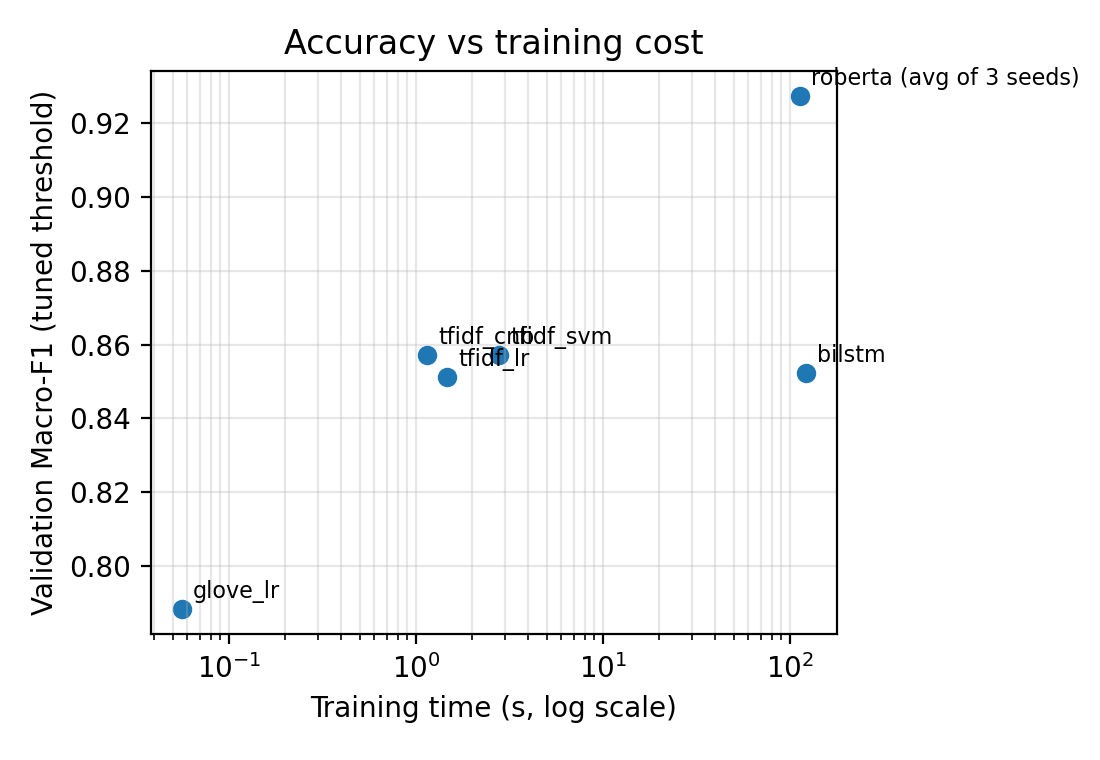
\includegraphics[width=0.62\textwidth]{f1_vs_train_time.png}
\caption{Validation Macro-F1 (tuned threshold) versus training time (log scale). Regenerated by \texttt{src/resource\_table.py} from every model's \texttt{metrics.json}. \tbd{final version after all outputs are in}}
\label{fig:g-scatter}
\end{figure}

\paragraph{Practical implications.}
\begin{itemize}
  \item \textbf{Small labelled data favours pre-trained features.} With only 5.9k training reviews, TF-IDF must learn every n-gram's polarity from scratch, and 24\% of the word types in the validation reviews never occur in training. Pre-trained embeddings, and above all pre-trained language models, bring knowledge learned from billions of words, so they generalise better to rare words, typos and paraphrases.
  \item \textbf{Large data or tight budgets favour sparse features.} TF-IDF scales linearly, runs on any CPU and is fully interpretable. It is the right choice when latency, cost or explainability matter more than the last percentage point, and it is a strong baseline.
  \item \textbf{Robustness to domain change differs.} TF-IDF and GloVe fix their vocabulary at training time. A subword model covers any input string, which matters for the hotel-review scenario in (h).
\end{itemize}
In short, for this task the feature format moves accuracy by a few points but cost by orders of magnitude. The choice should therefore follow the accuracy target and the available hardware.


\section{(h) Hotel reviews without rating scores}
% Owner: member B.
Hotel reviews share general cues such as \emph{excellent} and \emph{disappointing}
with product reviews, so a frozen source classifier provides a useful starting
point. The meaning of some features can change: \emph{small} can describe a
convenient electronic device or an uncomfortably small room. Hotel reviews also
discuss service, cleanliness and location, often with conflicting opinions in
the same review. Changes in the distribution of topics or class prevalence can
make the source-domain decision threshold poorly calibrated on hotel reviews.
Prior work on review transfer provides evidence for these risks, but the
magnitude of the loss on hotel reviews requires target-domain evaluation
\cite{blitzer2007biographies,karouzos2021udalm}.

\paragraph{Adaptation with raw hotel text.}
One option is to continue masked-language-model training on unlabeled hotel
reviews and then train the sentiment head on labeled product reviews. Another
is to train the sentiment head on source labels while using the hotel corpus
for a joint masked-language-model objective, as in UDALM~\cite{karouzos2021udalm}.
A cheaper alternative is self-training: label an unlabeled hotel pool with the
source model, retain only high-confidence examples from each predicted class,
and retrain with the original labeled reviews and a lower weight on pseudo-labels.
Confidence cutoffs should be conservative because domain shift can produce
confident errors and reinforce class imbalance. For a lightweight linear
model, structural correspondence learning can instead use frequent shared
pivot words to connect product and hotel vocabulary~\cite{blitzer2007biographies}.

\paragraph{Evaluation.}
If manual annotation is feasible, independently label a random sample of
approximately 100 hotel reviews using a fixed overall-polarity rubric.
Adjudicate disagreements and document how mixed or neutral reviews are treated.
Keep this set separate from the unlabeled adaptation pool. Compare the frozen
source model and adapted models on the same labeled reviews using accuracy,
Macro-F1 and negative-class F1. Any threshold chosen using hotel labels needs
a separate calibration set or a nested validation protocol. Without target
labels, inspect OOV rates and prediction distributions as diagnostics and
leave target-domain accuracy unreported.


\section{(i) Hotel reviews with noisy rating scores}
The question refers to ``the same sentiment classification problem in (g)''. We read this as the hotel-review project of (h): the reviews now come with rating scores, but some of those scores are wrong.
Training labels derived from the ratings are therefore \emph{noisy}.

\subsection*{How our classifier would be affected}

\paragraph{Sources and types of noise.}
Rating errors on review sites are rarely uniform~\cite{song2023learning}. Three kinds can be distinguished:
\begin{itemize}
  \item \emph{Random errors}, such as mis-clicks or swapped scales, are roughly \emph{symmetric}.
  \item \emph{Systematic errors} are \emph{class-conditional}. A guest may write a positive text but give a low score because of the price or a single incident, or a hotel may receive inflated scores. Noise then runs mainly in one direction.
  \item \emph{Instance-dependent errors} concentrate on ambiguous, mixed or sarcastic reviews, which are exactly the hard cases.
\end{itemize}

\paragraph{Effect on training.}
A discriminative classifier fits the labels it is given.
Over-parameterised neural networks can memorise even completely random labels. They do tend to learn the clean, dominant patterns first and only later fit the noise.
So a fine-tuned RoBERTa or a BiLSTM trained to convergence on noisy ratings would gradually absorb the errors, and its decision boundary and confidence estimates would suffer. Early stopping on clean data delays this but does not prevent it.
A regularised linear TF-IDF model cannot memorise as freely, but its weights are biased in the same way.
Class imbalance amplifies the damage. With an 85:15 class ratio, flipping each label independently with probability 20\% means only 41\% of the reviews labelled ``negative'' are truly negative, because flipped positives outnumber the real negatives.
The minority class, usually the one that matters most to a hotel, is affected first.

\paragraph{Effect on evaluation.}
If the validation and test labels are noisy too, measured accuracy underestimates the true accuracy, and model selection and threshold tuning chase the noise.
A small, manually verified clean set is therefore essential for any of the remedies below.

\subsection*{Experiment: injecting label noise into our data}
To quantify these effects we corrupted the labels of our 5{,}909 training-part reviews and kept the 1{,}492-review validation split clean.
We used two noise models:
\begin{itemize}
  \item \emph{symmetric}: every label is flipped with probability 0, 5, 10 or 20\%;
  \item \emph{positive$\to$negative}: only positive labels are flipped, with probability 5, 10 or 20\%, mimicking a positive text given a low score.
\end{itemize}
The base model is TF-IDF (word 1--2-grams) + LR, and each setting is repeated with 3 seeds.
Methods M1--M3 rely on 5-fold out-of-fold probabilities $p(x)$ computed on the noisy training part, with the same grouped folds as in (b). We compared four strategies:
\begin{itemize}
  \item \textbf{M0, baseline}: train on the noisy labels.
  \item \textbf{M1, sample selection (Confident Learning)}~\cite{northcutt2021confident}. For each class $j$, set the threshold $t_j$ to the mean predicted probability of $j$ over samples labelled $j$. A sample is flagged when its most probable class among those with $p_k \ge t_k$ differs from its given label. Flagged samples are removed and the model is retrained.
  \item \textbf{M2, label correction}: a label is flipped when the out-of-fold model assigns more than 0.9 probability to the opposite class.
  \item \textbf{M3, re-weighting}: each sample is weighted by the out-of-fold probability of its given label.
\end{itemize}

\begin{table}[t]
\centering
\caption{Validation results under injected label noise (mean $\pm$ std over 3 seeds). Left block: Macro-F1 at threshold~0.5. Right block: ROC-AUC, which does not depend on the threshold. ``Neg.\ prec.'' is the fraction of training reviews labelled negative that are truly negative. Without class weights and threshold tuning, the clean baseline's Macro-F1 (0.789) is lower than the tuned TF-IDF model in (g) (0.851).}
\label{tab:i-noise}
\small
\setlength{\tabcolsep}{3.5pt}
\begin{tabular}{l r c cccc cccc}
\toprule
 & & Neg. & \multicolumn{4}{c}{Macro-F1 @ 0.5} & \multicolumn{4}{c}{ROC-AUC} \\
\cmidrule(lr){4-7}\cmidrule(lr){8-11}
Noise & Rate & prec. & M0 & M1 & M2 & M3 & M0 & M1 & M2 & M3 \\
\midrule
--          & 0\%  & 1.00 & .789 & \textbf{.810} & .765 & .692 & \textbf{.950} & .948 & .946 & .945 \\
Symmetric   & 5\%  & 0.77 & .789 & \textbf{.814} & .789 & .698 & .938 & \textbf{.944} & \textbf{.944} & \textbf{.944} \\
            & 10\% & 0.60 & .772 & \textbf{.805} & .765 & .690 & .910 & .936 & .929 & \textbf{.939} \\
            & 20\% & 0.41 & .720 & \textbf{.792} & .754 & .724 & .837 & \textbf{.909} & .878 & .907 \\
Pos$\to$neg & 5\%  & 0.77 & .802 & \textbf{.823} & .812 & .728 & .935 & \textbf{.944} & \textbf{.944} & \textbf{.944} \\
            & 10\% & 0.63 & .806 & \textbf{.819} & .809 & .769 & .917 & .940 & .936 & \textbf{.941} \\
            & 20\% & 0.46 & .778 & \textbf{.819} & .796 & .814 & .901 & .931 & .917 & \textbf{.933} \\
\bottomrule
\end{tabular}\\[2pt]
\footnotesize Standard deviations are 0.003--0.020 for Macro-F1 and below 0.008 for AUC; full values are in \texttt{outputs/noise\_exp/summary.csv}.
\end{table}

\begin{figure}[t]
\centering
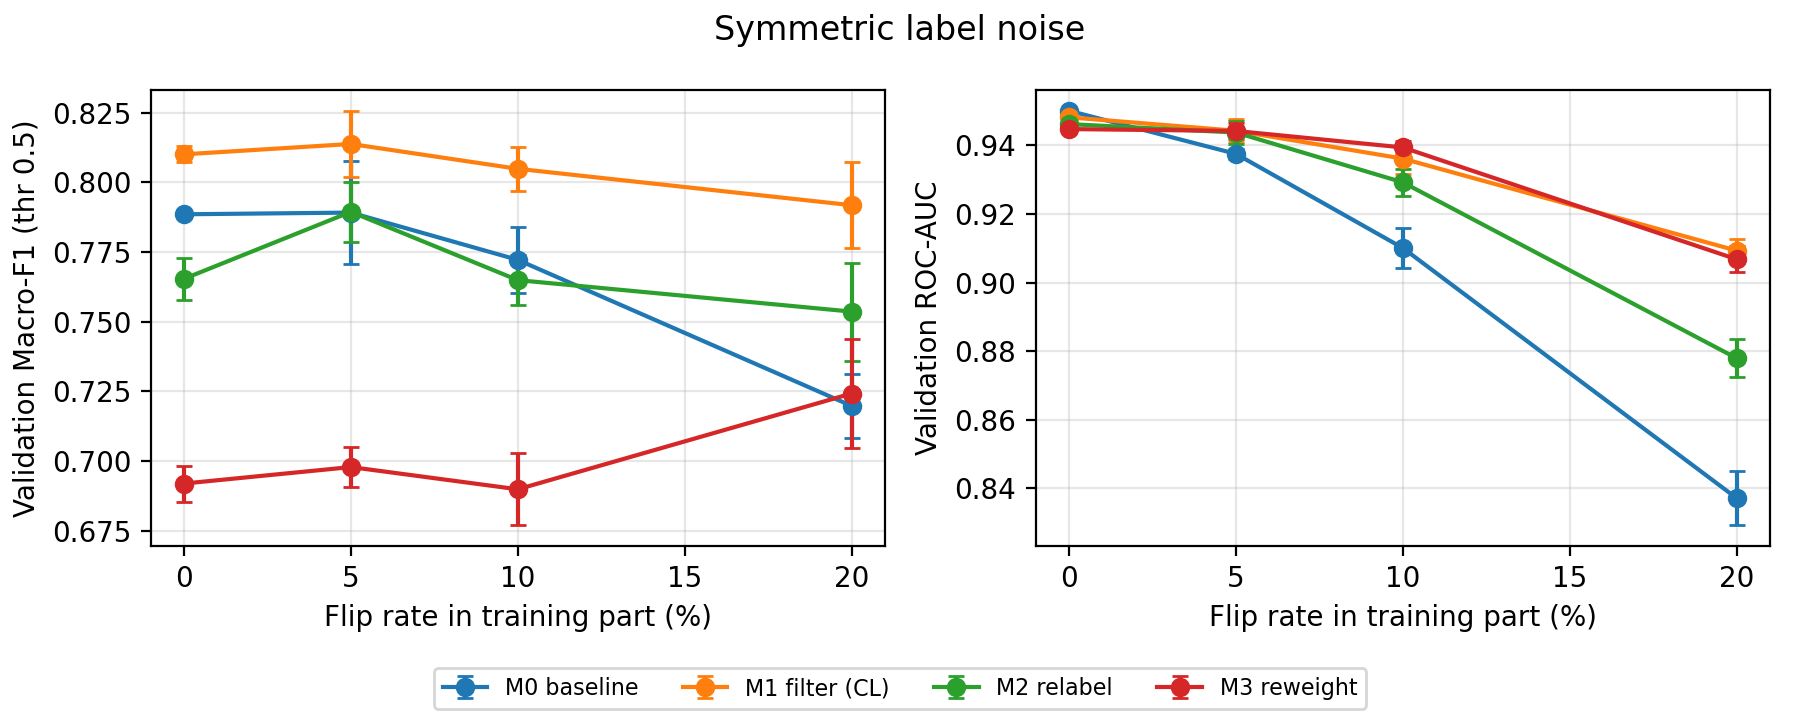
\includegraphics[width=\textwidth]{noise_symmetric.png}\\[4pt]
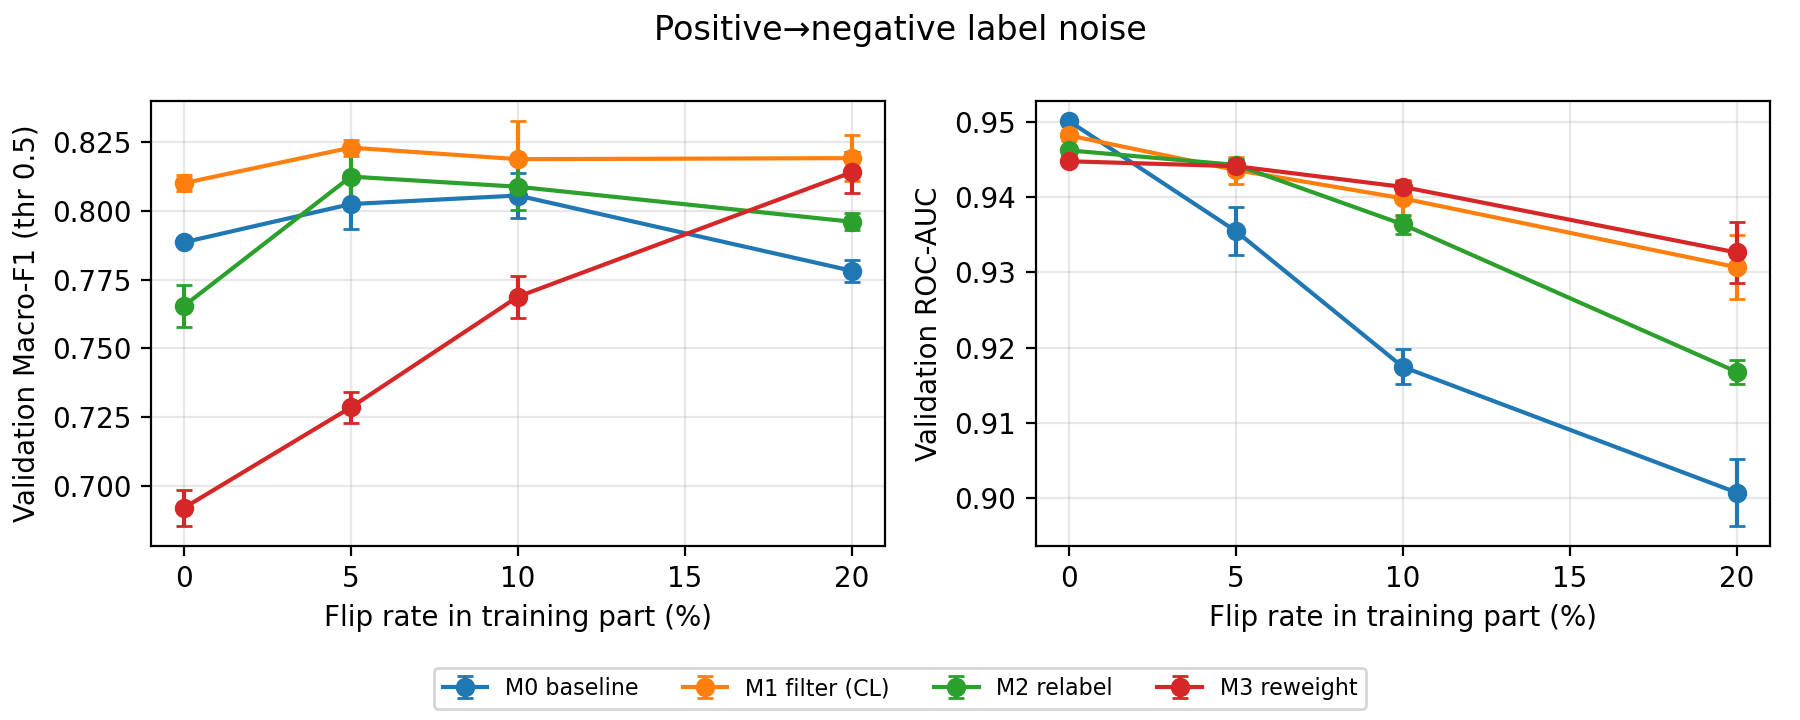
\includegraphics[width=\textwidth]{noise_pos2neg.png}
\caption{Validation Macro-F1 at threshold 0.5 (left) and ROC-AUC (right) as the training-label flip rate grows. Error bars show $\pm1$ std over 3 seeds.}
\label{fig:i-noise}
\end{figure}

\paragraph{Findings.}
Table~\ref{tab:i-noise} and Figure~\ref{fig:i-noise} lead to five observations.
\begin{enumerate}
  \item \textbf{Noise hurts, and imbalance makes it worse.} Under 20\% symmetric noise the baseline's AUC drops from 0.950 to 0.837, and its Macro-F1 from 0.789 to 0.720. The F1 of the negative class falls from 0.63 to 0.52.
  \item \textbf{Threshold-0.5 metrics can mislead.} Positive$\to$negative noise of 5--10\% slightly \emph{raises} the baseline's Macro-F1 at 0.5, although its AUC falls. The extra negative labels merely shift the decision boundary towards the minority class. This is why we also report AUC, and why thresholds must be tuned on clean data.
  \item \textbf{Sample selection (M1) is the most reliable method.} It gives the best Macro-F1 in every setting, and at 20\% symmetric noise it recovers AUC from 0.837 to 0.909. It removed 1{,}633 reviews on average; 44\% of them had actually been flipped, and it caught 61\% of all flipped labels. Even on the clean data it removed about 80 hard or ambiguous reviews and improved Macro-F1 by 0.02.
  \item \textbf{Label correction (M2) is precise but conservative.} 83--97\% of the labels it changed were truly wrong, but it changed only 200--280 of them, so its gains are moderate.
  \item \textbf{Re-weighting (M3) ranks well but needs re-calibration.} It matches M1 in AUC and is best under strong positive$\to$negative noise. However, its Macro-F1 at 0.5 is poor at low noise: negative reviews receive lower out-of-fold confidence, so re-weighting shrinks the minority class further. Combined with class weights or threshold tuning, this weakness would disappear.
\end{enumerate}
These results come from synthetic noise, a linear model and a single validation split. They show the size of the problem and the relative behaviour of the strategy families, not the gains to expect on real hotel ratings.

\subsection*{Three approaches to improve the algorithm}
The three families below follow the taxonomy of the recent survey by Song et al.~\cite{song2023learning}, where the individual methods named here are reviewed in detail.
\begin{enumerate}
  \item \textbf{Noise-robust losses and loss correction.} Replace plain cross-entropy with a loss that penalises confidently wrong labels less. Options include generalized cross-entropy, which interpolates between cross-entropy and the noise-tolerant MAE; symmetric cross-entropy; and label smoothing.
  When the noise is class-conditional, as with positive texts given low scores, one can instead estimate the $2\times2$ noise-transition matrix $T$ and correct the loss through it (forward/backward correction). $T$ can be estimated from a small clean subset.
  These methods change only the loss function of our RoBERTa fine-tuning, and add no extra cost.

  \item \textbf{Sample selection and data cleaning.} Exploit the fact that networks fit clean samples first, so small-loss samples are more likely to be correctly labelled.
  Co-teaching trains two networks and lets each one update on the small-loss samples chosen by the other. Confident Learning estimates the joint distribution of noisy and true labels from out-of-fold probabilities, then prunes or ranks the suspicious samples~\cite{northcutt2021confident}; this is our M1, the best method in our experiment.
  Flagged reviews can also be sent to annotators instead of being discarded.

  \item \textbf{Label correction and semi-supervised learning.} Instead of discarding suspicious samples, correct or down-weight them. Our M2 and M3 are simple versions.
  DivideMix fits a two-component mixture model to the per-sample losses to separate likely-clean from likely-noisy reviews. It then treats the noisy ones as \emph{unlabelled} data and trains on both parts with MixMatch-style semi-supervised learning.
  For hotel reviews, the text itself is a second, independent signal. A zero-shot model, for example our RoBERTa classifier or an LLM, can check each rating against its text, and the two can be combined into a corrected label.
\end{enumerate}

\paragraph{Recommended pipeline for the hotel project.}
\begin{enumerate}
  \item Manually verify a few hundred reviews to obtain a clean development set, and use it to estimate the noise rate and the transition matrix $T$.
  \item Fine-tune a pre-trained Transformer with a robust loss (GCE or label smoothing) and early stopping on the clean set.
  \item Run Confident Learning on out-of-fold predictions; relabel or drop the flagged reviews, sending the uncertain ones to annotators.
  \item Retrain, optionally with DivideMix-style semi-supervised learning on the doubtful part, and tune the decision threshold on the clean set.
\end{enumerate}


\appendix
\section{Code and instructions}
The code is in the \texttt{src/} folder. The project
\texttt{README.md} explains how to run the models and regenerate the
final predictions from the saved outputs.

\bibliographystyle{unsrtnat}
\bibliography{refs}
\end{document}
